\documentclass[tikz,border=4pt]{standalone}
\usepackage{pgfplots}
\pgfplotsset{compat=1.16}
\pgfplotsset{
  bode/.style={
    width=6.4cm, height=4.4cm, xmin=0.01, xmax=100,
    grid=both, major grid style={gray!55}, minor grid style={gray!20},
    tick label style={font=\footnotesize}, label style={font=\small},
    title style={font=\small}, xlabel={$\omega/\omega_z$},
  },
  bode mag/.style={bode, ymin=-50, ymax=50, ytick={-40,-20,0,20,40},
    ylabel={$|G|_{\mathrm{dB}}$}, title={Modulo}},
  bode fase/.style={bode, ymin=-100, ymax=100, ytick={-90,-45,0,45,90},
    ylabel={$\varphi$ [$^\circ$]}, title={Fase}},
}
\begin{document}
% G(j w) = 1 + j w/wz,  x = w/wz
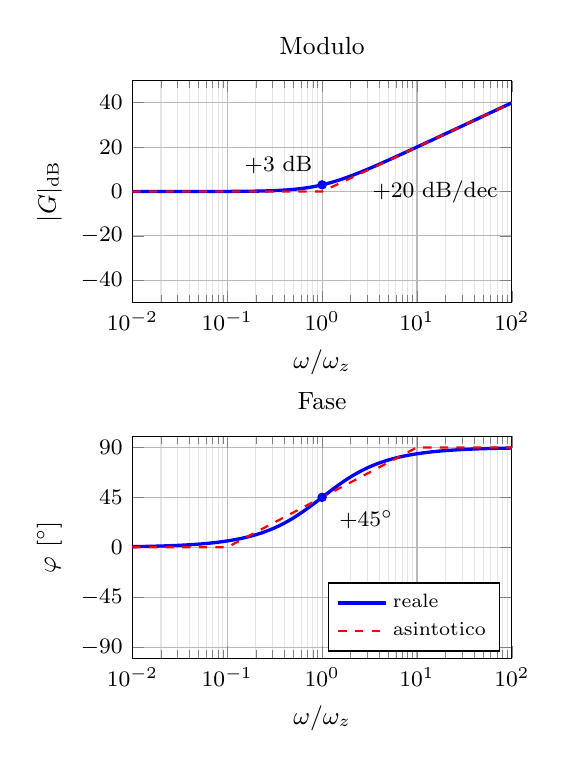
\begin{tikzpicture}
% ---------- modulo ----------
\begin{semilogxaxis}[bode mag, name=mag]
  \addplot[blue, very thick, domain=-2:2, samples=121] ({10^x}, {10*log10(1+10^(2*x))});
  \addplot[red, thick, dashed] coordinates {(0.01,0) (1,0) (100,40)};
  \addplot[only marks, mark=*, mark size=1.5pt, blue] coordinates {(1,3.01)};
  \node[anchor=south east, font=\footnotesize] at (axis cs:1,3.5) {$+3$ dB};
  \node[anchor=north east, font=\footnotesize] at (axis cs:90,9) {$+20$ dB/dec};
\end{semilogxaxis}
% ---------- fase ----------
\begin{semilogxaxis}[bode fase, at={(mag.south west)}, yshift=-1.7cm, anchor=north west,
  legend style={font=\scriptsize, at={(0.97,0.03)}, anchor=south east},
  legend cell align=left]
  \addplot[blue, very thick, domain=-2:2, samples=121] ({10^x}, {atan(10^x)});
  \addplot[red, thick, dashed] coordinates {(0.01,0) (0.1,0) (10,90) (100,90)};
  \legend{reale, asintotico}
  \addplot[only marks, mark=*, mark size=1.5pt, blue, forget plot] coordinates {(1,45)};
  \node[anchor=north west, font=\footnotesize] at (axis cs:1.2,42) {$+45^\circ$};
\end{semilogxaxis}
\end{tikzpicture}
\end{document}
